% Options for packages loaded elsewhere
\PassOptionsToPackage{unicode}{hyperref}
\PassOptionsToPackage{hyphens}{url}
\PassOptionsToPackage{dvipsnames,svgnames,x11names}{xcolor}
%
\documentclass[
]{report}

\usepackage{amsmath,amssymb}
\usepackage{iftex}
\ifPDFTeX
  \usepackage[T1]{fontenc}
  \usepackage[utf8]{inputenc}
  \usepackage{textcomp} % provide euro and other symbols
\else % if luatex or xetex
  \usepackage{unicode-math}
  \defaultfontfeatures{Scale=MatchLowercase}
  \defaultfontfeatures[\rmfamily]{Ligatures=TeX,Scale=1}
\fi
\usepackage{lmodern}
\ifPDFTeX\else  
    % xetex/luatex font selection
\fi
% Use upquote if available, for straight quotes in verbatim environments
\IfFileExists{upquote.sty}{\usepackage{upquote}}{}
\IfFileExists{microtype.sty}{% use microtype if available
  \usepackage[]{microtype}
  \UseMicrotypeSet[protrusion]{basicmath} % disable protrusion for tt fonts
}{}
\makeatletter
\@ifundefined{KOMAClassName}{% if non-KOMA class
  \IfFileExists{parskip.sty}{%
    \usepackage{parskip}
  }{% else
    \setlength{\parindent}{0pt}
    \setlength{\parskip}{6pt plus 2pt minus 1pt}}
}{% if KOMA class
  \KOMAoptions{parskip=half}}
\makeatother
\usepackage{xcolor}
\setlength{\emergencystretch}{3em} % prevent overfull lines
\setcounter{secnumdepth}{5}
% Make \paragraph and \subparagraph free-standing
\makeatletter
\ifx\paragraph\undefined\else
  \let\oldparagraph\paragraph
  \renewcommand{\paragraph}{
    \@ifstar
      \xxxParagraphStar
      \xxxParagraphNoStar
  }
  \newcommand{\xxxParagraphStar}[1]{\oldparagraph*{#1}\mbox{}}
  \newcommand{\xxxParagraphNoStar}[1]{\oldparagraph{#1}\mbox{}}
\fi
\ifx\subparagraph\undefined\else
  \let\oldsubparagraph\subparagraph
  \renewcommand{\subparagraph}{
    \@ifstar
      \xxxSubParagraphStar
      \xxxSubParagraphNoStar
  }
  \newcommand{\xxxSubParagraphStar}[1]{\oldsubparagraph*{#1}\mbox{}}
  \newcommand{\xxxSubParagraphNoStar}[1]{\oldsubparagraph{#1}\mbox{}}
\fi
\makeatother


\providecommand{\tightlist}{%
  \setlength{\itemsep}{0pt}\setlength{\parskip}{0pt}}\usepackage{longtable,booktabs,array}
\usepackage{calc} % for calculating minipage widths
% Correct order of tables after \paragraph or \subparagraph
\usepackage{etoolbox}
\makeatletter
\patchcmd\longtable{\par}{\if@noskipsec\mbox{}\fi\par}{}{}
\makeatother
% Allow footnotes in longtable head/foot
\IfFileExists{footnotehyper.sty}{\usepackage{footnotehyper}}{\usepackage{footnote}}
\makesavenoteenv{longtable}
\usepackage{graphicx}
\makeatletter
\def\maxwidth{\ifdim\Gin@nat@width>\linewidth\linewidth\else\Gin@nat@width\fi}
\def\maxheight{\ifdim\Gin@nat@height>\textheight\textheight\else\Gin@nat@height\fi}
\makeatother
% Scale images if necessary, so that they will not overflow the page
% margins by default, and it is still possible to overwrite the defaults
% using explicit options in \includegraphics[width, height, ...]{}
\setkeys{Gin}{width=\maxwidth,height=\maxheight,keepaspectratio}
% Set default figure placement to htbp
\makeatletter
\def\fps@figure{htbp}
\makeatother

\makeatletter
\@ifpackageloaded{caption}{}{\usepackage{caption}}
\AtBeginDocument{%
\ifdefined\contentsname
  \renewcommand*\contentsname{Table of contents}
\else
  \newcommand\contentsname{Table of contents}
\fi
\ifdefined\listfigurename
  \renewcommand*\listfigurename{List of Figures}
\else
  \newcommand\listfigurename{List of Figures}
\fi
\ifdefined\listtablename
  \renewcommand*\listtablename{List of Tables}
\else
  \newcommand\listtablename{List of Tables}
\fi
\ifdefined\figurename
  \renewcommand*\figurename{Figure}
\else
  \newcommand\figurename{Figure}
\fi
\ifdefined\tablename
  \renewcommand*\tablename{Table}
\else
  \newcommand\tablename{Table}
\fi
}
\@ifpackageloaded{float}{}{\usepackage{float}}
\floatstyle{ruled}
\@ifundefined{c@chapter}{\newfloat{codelisting}{h}{lop}}{\newfloat{codelisting}{h}{lop}[chapter]}
\floatname{codelisting}{Listing}
\newcommand*\listoflistings{\listof{codelisting}{List of Listings}}
\makeatother
\makeatletter
\makeatother
\makeatletter
\@ifpackageloaded{caption}{}{\usepackage{caption}}
\@ifpackageloaded{subcaption}{}{\usepackage{subcaption}}
\makeatother
\makeatletter
\@ifpackageloaded{sidenotes}{}{\usepackage{sidenotes}}
\@ifpackageloaded{marginnote}{}{\usepackage{marginnote}}
\makeatother

\ifLuaTeX
  \usepackage{selnolig}  % disable illegal ligatures
\fi
\usepackage[]{biblatex}
\addbibresource{references.bib}
\usepackage{bookmark}

\IfFileExists{xurl.sty}{\usepackage{xurl}}{} % add URL line breaks if available
\urlstyle{same} % disable monospaced font for URLs
\hypersetup{
  pdftitle={Tree object detection using airborne images and LiDAR point clouds},
  pdfauthor={Alexandre Bry},
  pdfkeywords={tree detection, deep learning},
  colorlinks=true,
  linkcolor={blue},
  filecolor={Maroon},
  citecolor={Blue},
  urlcolor={Blue},
  pdfcreator={LaTeX via pandoc}}


\title{Tree object detection using airborne images and LiDAR point
clouds}
\author{Alexandre Bry}
\date{2024-07-16}

\begin{document}
\maketitle
\begin{abstract}
This is the abstract. It can be on multiple lines and contain
\textbf{Markdown}.
\end{abstract}

\renewcommand*\contentsname{Table of contents}
{
\hypersetup{linkcolor=}
\setcounter{tocdepth}{2}
\tableofcontents
}

\chapter*{Introduction}\label{introduction}
\addcontentsline{toc}{chapter}{Introduction}

The goal of the internship was to study the possibility of combining
LiDAR point clouds and aerial images in a deep learning model to perform
instance segmentation of trees. The two types of data are indeed
complementary, as point clouds capture the shape of the worlds, while
images capture the colors. However, combining them into a format that
allows a model to handle them simultaneously is not an easy task because
they inherently have a very different spatial repartition and encoding.

The second major topic of the internship was to acquire a proper dataset
matching all the criteria required for the project. Most of the datasets
containing tree annotations only used either RGB images or LiDAR point
clouds, but not both. Therefore, I had to create such a dataset by
myself, using the openly available images and point clouds in the
Netherlands, by annotating trees by hand to properly train and evaluate
the methods.

\chapter{State-of-the-art}\label{state-of-the-art}

\section{Computer vision tasks related to
trees}\label{computer-vision-tasks-related-to-trees}

Before talking about models and datasets, let's define properly the task
that this project focused on, in the midst of all the various computer
vision tasks, and specifically those related to tree detection.

The first main differentiation between tree recognition tasks comes from
the acquisition of the data. There are some very different tasks and
methods using either ground data or aerial/satellite data. This is
especially true when focusing on urban trees, since a lot of street view
data is available \autocite{urban-trees}.

This leads to the second variation, which is related to the kind of tree
area that we are interested in. There are mainly three types of area,
which among other things, influence the organization of the trees in
space: urban areas, tree plantations and forests. This is important,
because the tasks and the difficulty depends on the type of area. Tree
plantations are much easier to work with than completely wild forests,
while urban areas contain various levels of difficulty ranging from
alignment trees to private and disorganized gardens and parks. For this
project, we mainly focused on urban areas, but everything should still
be applicable to tree plantations and forests.

Then, the four fundamental computer vision tasks have their application
when dealing with trees \autocite{olive-tree}:

\begin{itemize}
\tightlist
\item
  Classification, although this is quite rare for airborne tree
  applications since there are multiple trees on each image most of the
  time
\item
  Detection, which consists in detecting objects and placing boxes
  around them
\item
  Semantic segmentation, which consists in associating a label to every
  pixel of an image
\item
  Instance segmentation, which consists in adding a layer of complexity
  to semantic segmentation by also differentiating between the different
  instances of each class
\end{itemize}

These generic tasks can be extended by trying to get more information
about the trees. The most common information are the species and the
height, but some models also try to predict the health of the trees, or
their carbon stock.

In this paper, the task that is tackled is the detection of trees, with
a special classification between several labels related to the
discrepancies between the different kinds of data. The kind of model
that is used would also have allowed to focus on some more advanced
tasks, by replacing detection with instance segmentation and asking the
model to also predict the species. But due to the difficulties regarding
the dataset, a simpler task with a simpler dataset was used, without
compromising the ability to experiment with different possible
improvements of the model. The difficulties and the experiments are
developed below.

\section{Datasets}\label{datasets}

\subsection{Motivations}\label{motivations}

\autocite{lidar_benchmark_2} shows that in forests, you can have up to
more than 50\% of the trees which crowns are completely or partially
covered by other trees.

\subsection{Requirements}\label{requirements}

Before presenting the different promising datasets and the reasons why
they were not fully usable for the project, let's enumerate the
different conditions and requirements for the tree instance segmentation
task:

\begin{itemize}
\tightlist
\item
  Multiple types of data:

  \begin{itemize}
  \tightlist
  \item
    Aerial RGB images
  \item
    LiDAR point clouds (preferably aerial)
  \item
    (Optional) Aerial infrared images
  \end{itemize}
\item
  Tree crown annotations or bounding boxes
\item
  High-enough resolution:

  \begin{itemize}
  \tightlist
  \item
    For images, about 25~cm
  \item
    For point clouds, about 10~cm
  \end{itemize}
\end{itemize}

Here are the explanations for these requirements. As for the types of
data, RGB images and point clouds are required to experiment on the
ability of the model to combine the two very different kinds of
information they hold. Having infrared data as well could be beneficial,
but it was not necessary. Regarding tree annotations, it was necessary
to have a way to spatially identify them individually, using crown
contours or simply bounding boxes. Since the model outputs bounding
boxes, any kind of other format could easily be transformed to bounding
boxes. Finally, the resolution had to be high enough to identify
individual trees and be able to really use the data. For the point
clouds especially, the whole idea was to see if and how the topology of
the trees could be learnt, using at least the trunks and even the
biggest branches if possible. Therefore, even if they are not really
comparable, this is the reason why the required resolution is more
precise for the point clouds.

Unfortunately, none of the datasets that I found matched all these
criteria. Furthermore, I didn't find any overlapping datasets that I
could merge to create a dataset with all the required types of data. In
the next parts, I will go through the different kinds of datasets that
exist, the reasons why they did not really fit for the project and the
ideas I got when searching for a way to use them.

\subsection{Existing tree datasets}\label{existing-tree-datasets}

As explained above, there were quite a lot of requirements to fulfill to
have a complete dataset usable for the task. This means that almost all
the available datasets were missing something, as they were mainly
focusing on using one kind of data and trying to make the most out of
it, instead of trying to use all the types of data together.

The most comprehensive list of tree annotations datasets was published
in OpenForest \autocite{OpenForest}. FoMo-Bench \autocite{FoMo-Bench}
also lists several interesting datasets, even though most of them can
also be found in OpenForest. Without enumerating all of them, there were
multiple kinds of datasets that all have their own flaws regarding the
requirements I was looking for.

Firstly, there are the forest inventories. TALLO \autocite{TALLO} is
probably the most interesting one in this category, because it contains
a lot of spatial information about almost 500K trees, with their
locations, their crown radii and their heights. Therefore, everything
needed to localize trees is in the dataset. However, I didn't manage to
find RGB images or LiDAR point clouds of the areas where the trees are
located, making it impossible to use these annotations to train tree
detection.

Secondly, there are the RGB datasets. ReforesTree \autocite{ReforesTree}
and MillionTrees \autocite{MillionTrees} are two of them and the quality
of their images are high. The only drawback of these datasets is
obviously that they don't provide any kind of point cloud, which make
them unsuitable for the task.

Thirdly, there are the LiDAR datasets, such as \autocite{WildForest3D}
and \autocite{FOR-instance}. Similarly to RGB datasets, they lack one of
the data source for the task I worked on. But unlike them, they have the
advantage that the missing data could be much easier to acquire from
another source, since RGB aerial or satellite images are much more
common than LiDAR point clouds. However, this solution was abandoned for
two main reasons. First it is quite challenging to find the exact
locations where the point clouds were acquired. Then, even when the
location is known, it is often in the middle of a forest where the
quality of satellite imagery is very low.

Finally, I also found two datasets that had RGB and LiDAR components.
The first one is MDAS \autocite{MDAS}. This benchmark dataset
encompasses RGB images, hyperspectral images and Digital Surface Models
(DSM). There were however two major flaws. The obvious one was that this
dataset was created with land semantic segmentation tasks in mind, so
there was no tree annotations. The less obvious one was that a DSM is
not a point cloud, even though it is some kind of 3D information and was
often created using a LiDAR point cloud. As a consequence, I would have
been very limited in my ability to use the point cloud.

The only real dataset with RGB and LiDAR came from NEON
\autocite{NEONdata}. This dataset contains exactly all the data I was
looking for, with RGB images, hyperspectral images and LiDAR point
clouds. With 30975 tree annotations, it is also a quite large dataset,
spanning across multiple various forests. The reason why I decided not
to use it despite all this is that at the beginning of the project, I
thought that the quality of the images and the point clouds was too low.
Looking back on this decision, I think that I probably could have worked
with this dataset and gotten great results. This would have saved me the
time spent annotating the trees for my own dataset, which I will talk
more about later. My decision was also influenced by the quality of the
images and the point clouds available in the Netherlands, which I will
talk about in the next section.

\subsection{Public data}\label{public-data}

After rejecting all the available datasets I had found, the only
solution I had left was to create my own dataset. I won't dive too much
in this process that I will explain in Section~\ref{sec-dataset}. I just
want to mention all the publicly available datasets that I used or could
have used to create this custom dataset.

For practical reasons, the two countries where I mostly searched for
available data are France and the Netherlands. I was looking for three
different data types independently:

\begin{itemize}
\tightlist
\item
  RGB (and eventually infrared) images
\item
  LiDAR point clouds
\item
  Tree annotations
\end{itemize}

These three types of data are available in similar ways in both
countries, although the Netherlands have a small edge over France. RGB
images are really easy to find in France with the BD ORTHO
\autocite{IGN_BDORTHO} and in the Netherlands with the Luchtfotos
\autocite{Luchtfotos}, but the resolution is better in the Netherlands
(8~cm vs 20~cm). Hyperspectral images are also available in both
countries, although for those the resolution is only 25~cm in the
Netherlands.

As for LiDAR point clouds, the Netherlands have a small edge over
France, because they have already completed their forth version covering
the whole country with AHN4 \autocite{AHN4}, and are working on the
fifth version. In France, data acquisition for the first LiDAR point
cloud covering the whole country started a few years ago
\autocite{IGN_LiDARHD}. It is not yet finished, even though data is
already available for half of the country. The other advantage of the
data from Netherlands regarding LiDAR point clouds is that all flights
are performed during winter, which allows light beams to penetrate more
deeply in trees and reach trunks and branches. This is not the case in
France.

The part that is missing in both countries is related to tree
annotations. Many municipalities have datasets containing information
about all the public trees they handle. This is for example the case for
Amsterdam \autocite{amsterdam_trees} and Bordeaux
\autocite{bordeaux_trees}. However, these datasets cannot really be used
as ground truth for a custom dataset for several reasons. First, many of
them do not contain coordinates indicating the position of each tree in
the city. Then, even those that contain coordinates are most of the time
missing any kind of information allowing to deduce a bounding box for
the tree crowns. Finally, even if they did contain everything, they only
focus on public trees, and are missing every single tree located in a
private area. Since public and private areas are obviously imbricated in
all cities, it means that any area we try to train the model on would be
missing all the private trees, making the training process impossible
because we cannot have only a partial annotation of images.

The other tree annotation source that we could have used is Boomregister
\autocite{boomregister}. This work covers the whole of the Netherlands,
including public and private trees. However, the precision of the masks
is far from perfect, and many trees are missing or incorrectly
segmented, especially when they are less than 9~m heigh or have a crown
diameter smaller than 4~m. Therefore, even it is a very impressive piece
of work, we thought that it could not be used as training data for a
deep learning models due to its biases and imperfections.

\subsection{Dataset augmentation
techniques}\label{dataset-augmentation-techniques}

When a dataset is too small to train a model, there are several ways of
artificially enlarging it.

The most common way to do it is to randomly apply deterministic or
random transformations to the data, during the training process, to be
able to generate several unique and different realistic data instances
from one real data instance. There are a lot of different
transformations that can be applied to images, divided into two
categories: pixel-level and spatial-level \autocite{albumentations}.
Pixel-level transformations modify the value of individual pixels, by
applying different filters, such as random noise, color shifts and more
complex effects like fog and sun flare. Spatial-level transformations
modify the spatial arrangement of the image, without changing the pixel
values. In other words, these transformations move the pixels in the
image. The transformations range from simple rotations and croppings to
complex spatial distortions. In the end, all these transformations are
simply producing one artificial image out of one real image.

Another way to enlarge a dataset is to instead generate completely new
input data sharing the same properties as the initial dataset. This can
be done using Generative Adversarial Networks (GAN). These models
usually have two parts, a generator and a discriminator, which are
trained in parallel. The generator learns to produce realistic
artificial data, while the discriminator learns to identify real data
and artificial data produced by the generator. If the training is
successful, we can then use the generator and random seeds to generate
random but realistic artificial data similar to the dataset. This method
has for example been successfully used to generate artificial tree
height maps \autocite{gan_data_augment}.

\section{Models and methods}\label{models-and-methods}

\subsection{Classical methods}\label{classical-methods}

Besides machine and deep learning methods that are mentioned in the next
sections, there exist several algorithmic methods that use the special
shape of the trees to detect them individually. The most used is called
the watershed algorithm, and even though it has many variants, its base
principle is simple \autocite{watershed}. The idea of this algorithm is
to find individual trees in three steps:

\begin{enumerate}
\def\labelenumi{\arabic{enumi}.}
\tightlist
\item
  Identify the local treetops from a height map or from an RGB image,
\item
  Inverse the image so that local maxima (treetops) become local minima
  (watersheds),
\item
  Fill the watersheds with water until different watersheds overflow and
  merge, marking their boundaries.
\end{enumerate}

This algorithm works generally well, using the assumption that the
overall shape of each individual tree crown si similar to a cone when
seen from above. Due to its success and the different changes that
further improved its results, this algorithm is still used today, even
in complex pipelines using machine and deep learning methods to extract
features before applying the watershed algorithm
\autocite{Freudenberg2022,lidar_rgb_wst}.

\subsection{LiDAR only}\label{lidar-only}

Some of the methods to identify individual trees use LiDAR data only.
There are a lot of different ways to use and analyze point clouds, but
the one that is mostly used for trees is based on height maps, or Canopy
Height Models (CHM).

A CHM is a raster computed as the subtraction of the Digital Terrain
Model (DTM) to the Digital Surface Model (DSM). What it means is that a
CHM contains the height above ground of the highest point in the area
corresponding to each pixel. This CHM can for example be used as the
input raster for the watershed algorithm, as it contains the height
values that can be used to determine local maxima
\autocite{lidar_watershed}.

\subsection{Images only}\label{images-only}

\subsection{LiDAR and images}\label{lidar-and-images}

Models to cite:

\begin{itemize}
\tightlist
\item
  AMF GD YOLOv8 \autocite{amf_gd_yolov8}: main source of inspiration,
  combining RGB and LiDAR in an image model
\item
  Benchmark of 8 methods using LiDAR \autocite{lidar_benchmark}: no
  machine learning method, but one of the methods uses multiple CHM
  layers, computed iteratively by removing everything in the 0.5~m below
  the previous CHM
\item
  Individual tree crown delineation in high-resolution remote sensing
  images based on U-Net \autocite{Freudenberg2022}: multiple steps with
  two models to predict masks, outlines and distance transform, and a
  final step with the watershed algorithm
\item
  DeepForest: A Python package for RGB deep learning tree crown
  delineation \autocite{DeepForest}: uses only RGB data to detect trees,
  but uses LiDAR to create millions of annotations of moderate quality
  to pre-train the model, before using around 10,000 hand-annotations to
  finalize and specialize the training on a certain area.
\item
  International Benchmarking of the Individual Tree Detection Methods
  for Modeling 3-D Canopy Structure for Silviculture and Forest Ecology
  Using Airborne Laser Scanning \autocite{lidar_benchmark_2}: another
  benchmark using LiDAR. They also try a method based on 3D voxels.
\item
  Deep Learning for LiDAR Point Cloud Classification in Remote Sensing
  \autocite{lidar_classification}: overview of deep learning methods to
  classify point clouds
\item
  Individual tree segmentation and tree species classification in
  subtropical broadleaf forests using UAV-based LiDAR, hyperspectral,
  and ultrahigh-resolution RGB data \autocite{lidar_rgb_wst}: use LiDAR,
  RGB and hyperspectral data, watershed algorithm and random forests.
\item
  ACE R-CNN: An Attention Complementary and Edge Detection-Based
  Instance Segmentation Algorithm for Individual Tree Species
  Identification Using UAV RGB Images and LiDAR Data
  \autocite{lidar_rgb_acnet}: use LiDAR and RGB data, Mask R-CNN model
  with fusion, similar to AMF GD YOLOv8
\end{itemize}

\chapter{Dataset}\label{sec-dataset}

The highest resolution of the CHM which keeps a high enough quality
depends entirely on the density of the point cloud. Also, depending on
the season when the point cloud is acquired, using a CHM might imply
throwing away the majority of the information contained in the point
cloud.

\section{Definition and content}\label{definition-and-content}

\section{Challenges}\label{challenges}

\begin{itemize}
\tightlist
\item
  Shift between RGB images, CIR images and LiDAR point clouds due to
  images not being perfectly orthonormal
\item
  Variations of the trees over time, with new small trees being planted
  and old trees being cut off
\item
  Not so easy to define what we consider as a tree and identify them.
  Problems with bushes for example. This problem is also mentioned in
  another paper \autocite{DeepForestBefore}.
\end{itemize}

\section{Augmentation methods}\label{augmentation-methods}

\chapter{Model}\label{model}

\chapter{Results}\label{results}

sortedAP: \autocite{sortedAP}.

\begin{figure*}[H]

\centering{

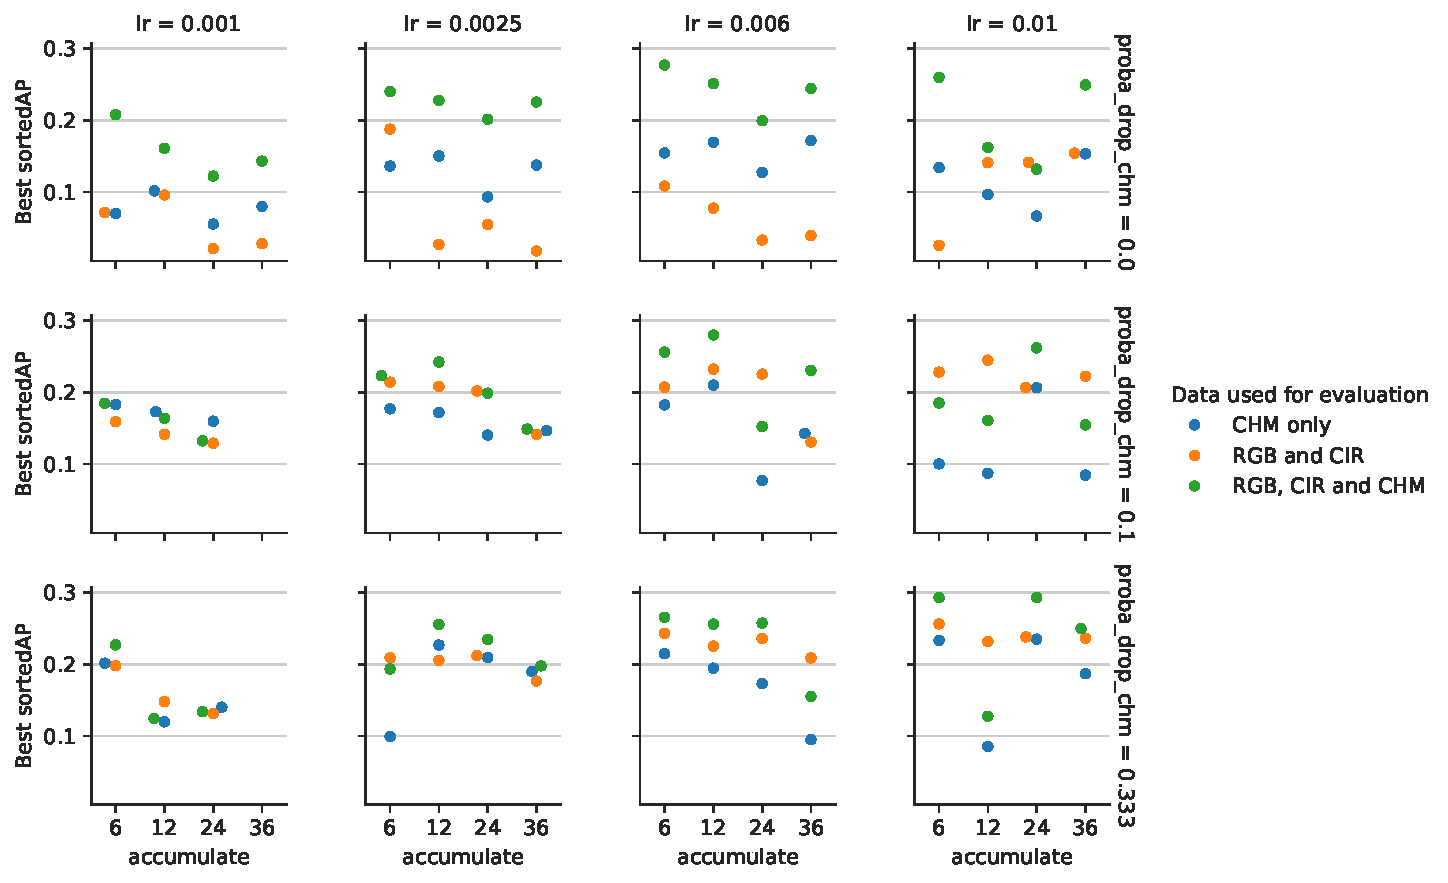
\includegraphics{index_files/figure-pdf/fig-training-parameters-output-1.pdf}

}

\caption{\label{fig-training-parameters}Results with different training
parameters}

\end{figure*}%

\begin{figure*}

\textsubscript{Source:
\href{https://ZokszY.github.io/Geodan-internship-report/index-preview.html}{Article
Notebook}}

\end{figure*}%

\chapter*{Conclusion}\label{conclusion}
\addcontentsline{toc}{chapter}{Conclusion}

Blablabla

\textsubscript{Source:
\href{https://ZokszY.github.io/Geodan-internship-report/index-preview.html}{Article
Notebook}}


\printbibliography[title=Bibliography]



\end{document}
